% Chapter 3

% --- Macro \xvec
\makeatletter
\newlength\xvec@height%
\newlength\xvec@depth%
\newlength\xvec@width%
\newcommand{\xvec}[2][]{%
  \ifmmode%
    \settoheight{\xvec@height}{$#2$}%
    \settodepth{\xvec@depth}{$#2$}%
    \settowidth{\xvec@width}{$#2$}%
  \else%
    \settoheight{\xvec@height}{#2}%
    \settodepth{\xvec@depth}{#2}%
    \settowidth{\xvec@width}{#2}%
  \fi%
  \def\xvec@arg{#1}%
  \def\xvec@dd{:}%
  \def\xvec@d{.}%
  \raisebox{.2ex}{\raisebox{\xvec@height}{\rlap{%
    \kern.05em%  (Because left edge of drawing is at .05em)
    \begin{tikzpicture}[scale=1]
    \pgfsetroundcap
    \draw (.05em,0)--(\xvec@width-.05em,0);
    \draw (\xvec@width-.05em,0)--(\xvec@width-.15em, .075em);
    \draw (\xvec@width-.05em,0)--(\xvec@width-.15em,-.075em);
    \ifx\xvec@arg\xvec@d%
      \fill(\xvec@width*.45,.5ex) circle (.5pt);%
    \else\ifx\xvec@arg\xvec@dd%
      \fill(\xvec@width*.30,.5ex) circle (.5pt);%
      \fill(\xvec@width*.65,.5ex) circle (.5pt);%
    \fi\fi%
    \end{tikzpicture}%
  }}}%
  #2%
}
\makeatother

% --- Override \vec with an invocation of \xvec.
\let\stdvec\vec
\renewcommand{\vec}[1]{\xvec[]{#1}}
% --- Define \dvec and \ddvec for dotted and double-dotted vectors.
\newcommand{\dvec}[1]{\xvec[.]{#1}}
\newcommand{\ddvec}[1]{\xvec[:]{#1}}

\chapter{Concetti di animazione} 

\label{Chapter3} % For referencing this chapter elsewhere, use \ref{ChapterX}

Animare significa "muovere" un modello, altrimenti statico, nel tempo. Questi movimenti sono definiti attraverso delle trasformazioni geometriche (traslazione, rotazione e scalatura).
Di seguito vengono riportate alcune tecniche di animazione 3D, spiegandone le metodologie, i pregi, i difetti e il contesto in cui possono venire utilizzate. 


\section{Rappresentazioni di rotazione}\label{Section3.1}
Lo scopo di questo paragrafo è descrivere le possibili rappresentazioni matematiche di una rotazione.
Alcuni di questi concetti sono validi anche per altre trasformazioni.
Tuttavia verranno considerate soltanto le rotazioni, in quanto queste ultime sono uno degli aspetti principali nella realizzazione di animazioni --- in particolare di animazioni 3D --- e alla base di alcune tecniche di animazione --- \emph{Inverse Kinematics} (IK) --- come anche uno dei più complessi. 

Come vedremo in seguito sarà indispensabile capire quale delle seguenti rappresentazioni conviene utilizzare in base all'animazione che si vuole realizzare.


\subsection{Angolo-asse}
Questo tipo di rappresentazione è senza dubbio la più semplice.
Utilizza 4 valori: 3 per specificare l'asse, ed 1 per l'angolo.
In questo modo, con una singola rotazione, è possibile raggiungere qualsiasi orientamento dell'oggetto che si sta ruotando.
Così come esiste sempre una linea retta che collega due punti nello spazio, si può pensare ad una rotazione angolo-asse come una singola rotazione che collega due orientamenti.

Questa rappresentazione è ottima per rotazioni di articolazioni con un solo \emph{Degree Of Freedom} (DOF).
È anche possibile definire articolazioni con più di un DOF semplicemente concatenando $n$ articolazioni su singolo asse connesse da $n-1$ ossa (i.e. oggetti connessi in un'articolazione) di lunghezza 0.
Ciò però rende la giuntura risultante inutilmente complessa da animare.
Per questo motivo le rappresentazione con angoli di Eulero, o sotto forma di quaternione, sono quelle più spesso utilizzate.
Inoltre la rappresentazione dell'asse attraverso 3 componenti numeriche non risulta di facile comprensione per l'utente che di solito preferisce usare quella Euleriana anche per rotazioni su singolo asse.

\subsection{Euleriana}

\begin{figure}
\centering
\begin{subfigure}{.5\textwidth}
  \centering
  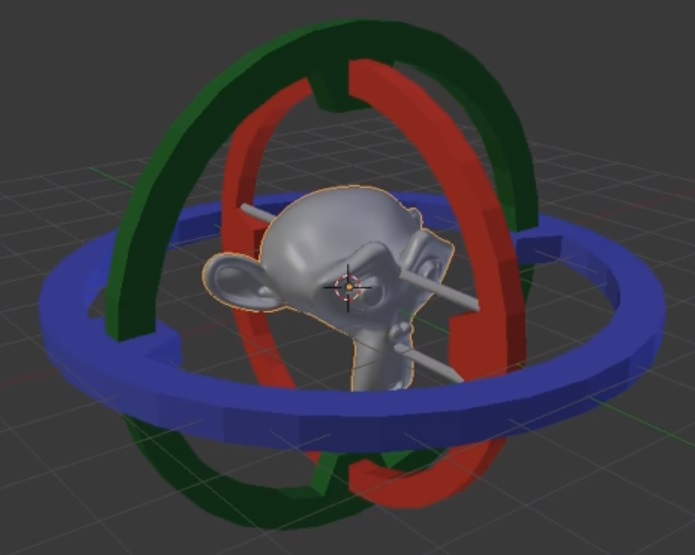
\includegraphics[width=.9\linewidth]{Figures/euler-1.jpg}
  \caption{Posizione neutra.}
  \label{fig:eulerA}
\end{subfigure}%
\begin{subfigure}{.5\textwidth}
  \centering
  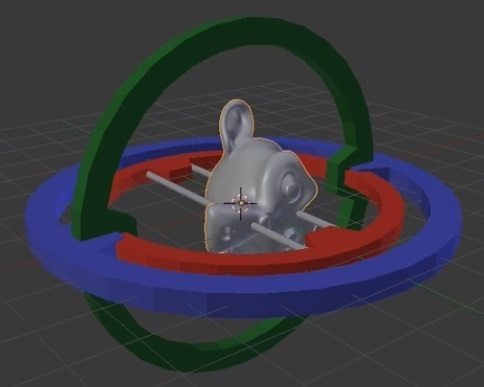
\includegraphics[width=.9\linewidth]{Figures/euler-2.jpg}
  \caption{Gimbal lock, l'asse X e Z sono allineati.}
  \label{fig:eulerB}
\end{subfigure}\\[2ex]
  \begin{minipage}{\textwidth}
  \footnotesize
  \emph{(Immagini di Nathan Vegdahl)}
  \end{minipage}
\decoRule
\caption[Rotazione Euleriana]{Rappresentazione di rotazione Euleriana attraverso un giroscopio a tre assi.}
\label{fig:euler}
\end{figure}

Concettualmente è la più intuitiva di tutte: utilizza 3 assi di rotazione (X, Y, Z) ed il funzionamento è analogo a quello di un giroscopio. Ogni asse offre un DOF, quindi sono possibili rotazioni con 3 DOF. Tuttavia sono necessarie due accortezze: 
\begin{enumerate}
    \item ordine degli assi;
    \item gimbal lock problem.
\end{enumerate}
L'ordine degli assi è decisivo, in quanto quello più interno dipende dalla rotazione di quelli esterni.
Di conseguenza ruotando gli assi in un ordine diverso da quello specificato porta a risultati diversi da quello atteso.
In più, interpolazioni tra diversi orientamenti, possono a loro volta risultare sgradevoli, poiché la rotazione viene spezzata in 3 movimenti.

Il problema del gimbal lock \parencite{anticz16}, in italiano blocco cardanico, sorge dall'allineamento di due assi: quello più interno e quello più esterno.
Ne deriva che ruotando uno di questi 2 assi si ottiene la stessa rotazione, perdendo quindi un DOF.
È quindi importante scegliere l'ordine degli assi in maniera tale che il primo e il terzo non risultino mai allineati.

Per ovviare a questo problema può essere conveniente bloccare uno degli assi in una posizione fissa. Per questo motivo, la forma Euleriana è meglio utilizzata nelle giunture con 1 o 2 DOF.

\newpage
\subsection{Quaternione}
\begin{figure}[ht]
\centering
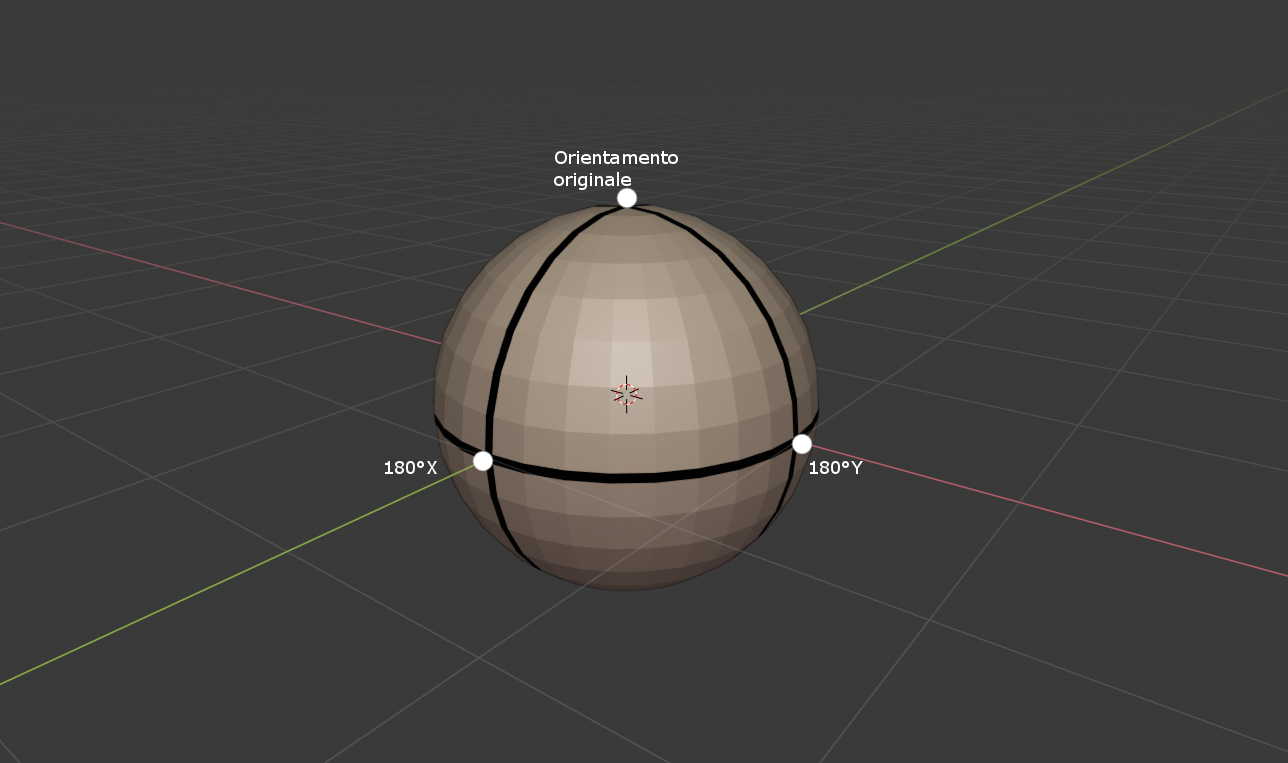
\includegraphics[width=.8\textwidth]{Figures/3d-sphere}
\decoRule
\caption[Quaternione 2D]{Rappresentazione di un quaternione 2D su una sfera 3D.}
\label{fig:quater}
\end{figure}
Diversamente da quanto appena visto, la forma di quaternione è concettualmente complessa, ma in pratica diventa molto utile e senza molti dei difetti della controparte Euleriana.

I principali benefici della rappresentazione a quaternione includono l'eliminazione del gimbal lock.
Infatti è presente una componente in più, ma ciascuna componente non rappresenta un asse quanto piuttosto l'orientamento dell'oggetto ruotato intorno a quell'asse.
La quarta componente serve, quindi, a definire la posizione neutra.

L'interpolazione risulta diretta e dolce, infatti il movimento non è spezzato sui diversi assi e l'ordine di questi non è importante.
Infine rende comodo calcolare una rotazione opposta semplicemente invertendo il segno della componente W.

Per rendere tutto ciò possibile servono 4 componenti (X, Y, Z, W), come già detto in precedenza, una per la posizione originale più una per la rotazione su ogni asse. Se si prende il caso di rotazioni su due assi si può immaginare che queste 3 componenti siano 3 punti su una sfera, come mostrato in Figura \ref{fig:quater}. Ogni altra rotazione è data dall'interpolazione di questi tre punti.

La ragione per cui i due punti sulla sfera rappresentano una rotazione di 180\textdegree\ anziché 90\textdegree\ è resa necessaria in quanto, altrimenti, questi due punti coinciderebbero nel punto più basso della sfera.
Come effetto aggiuntivo è possibile rappresentare rotazioni fino a 720\textdegree\ ed ogni orientamento equivale a due possibili rotazioni dando all'animatore l'abilità di decidere in che verso ruotare l'oggetto durante un'animazione.


\subsection{Matriciale}
Quest'ultima è probabilmente la rappresentazione più ottimale in termini di flessibilità, in quanto permette di rappresentare anche traslazioni, scalature e altre trasformazioni come \emph{shear}.
È, infatti, la rappresentazione che Blender utilizza internamente \cite{blendApi} \cite{nat2012rig} proprio perché offre la maggior flessibilità.

Siccome permette di rappresentare qualsiasi tipo di trasformazione, questa struttura viene solitamente chiamata \emph{Matrice di Trasformazione}. Nel caso di uno spazio a 3 dimensioni, essa ha dimensione $4\times4$.

Questa sua caratteristica la rende indispensabile per rappresentare articolazioni formate da più ossa (i.e Kinematics Linkages), che verranno illustrate qui di seguito (sezioni \ref{sectionFK} e \ref{sectionIK}), poiché rende possibile convertire le coordinate locali di un osso (rappresentato in Figura \ref{fig:FK}, evidenziato in azzurro) figlio a quelle locali del suo padre, fino ad arrivare alle coordinate globali.

L'unico difetto è che, come la rappresentazione sotto forma di quaternione, non mantiene l'informazione sul percorso della rotazione. Infatti è ancora più simile a una delta-rotazione (i.e. differenza di orientamento), rispetto ad un quaternione poiché copre una rotazione di soli 360\textdegree, rispetto ai 720\textdegree\ del quaternione. 

\newpage
\section{Cinematica Diretta} \label{sectionFK}

\begin{figure}
\centering
\begin{subfigure}{.33\textwidth}
  \centering
  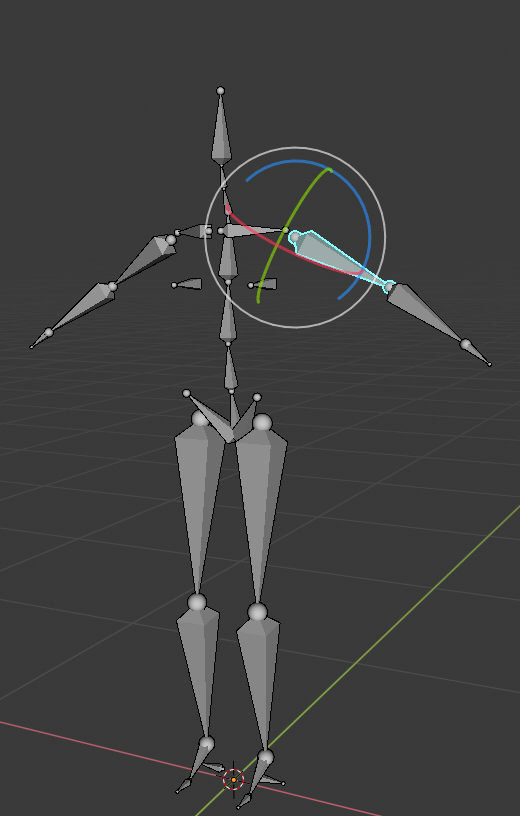
\includegraphics[width=\linewidth]{Figures/armature1}
  \label{fig:FK1}
\end{subfigure}%
\begin{subfigure}{.33\textwidth}
  \centering
  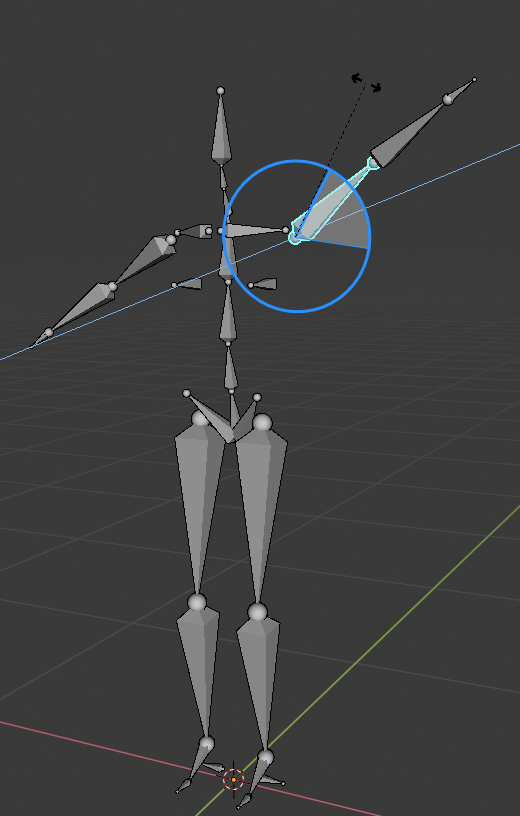
\includegraphics[width=\linewidth]{Figures/armature2}
  \label{fig:FK2}
\end{subfigure}%
\begin{subfigure}{.33\textwidth}
  \centering
  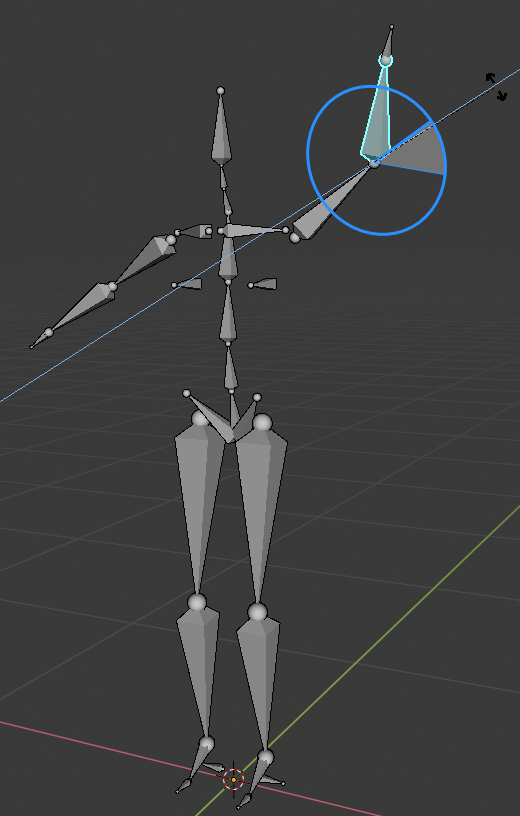
\includegraphics[width=\linewidth]{Figures/armature3}
  \label{fig:FK3}
\end{subfigure}
\decoRule
\caption[Cinematica Diretta]{Esempio di posizionamento tramite Forward Kinematic. La figura rappresenta la stessa armatura, formata da diverse ossa, in tre posizioni differenti.}
\label{fig:FK}
\end{figure}

Per figure complesse, come quella umana (da qui in avanti tutti gli esempi saranno riferiti alla figura umana, siccome, nella realizzazione del corto, è stata il centro della maggior parte delle animazioni), è utile avere un sistema che permetta di posizionare le sue componenti in maniera relativa ad altre.
Per esempio, una volta posizionato il busto, posizionare il braccio, poi la mano ed infine le dita, tutto in maniera relativa a quanto posizionato in precedenza.

Questa tecnica permette infatti di specificare, attraverso una rotazione, la posizione di un osso relativa al suo osso padre.
Per questo motivo è necessario che le ossa di un'armatura (vedi Figura \ref{fig:FK}) siano organizzate in maniera gerarchica (i.e. ad albero).
In questo modo, quando l'armatura viene posizionata basterà moltiplicare tutte le matrici di trasformazione dalla radice ai nodi foglia in maniera \emph{deep-first}. 
Per definire una posa è quindi necessario specificare la rotazione di ogni osso. Questo permette un controllo preciso su ogni DOF dell'armatura, il che è ottimo, perché permette all'animatore di realizzare pose perfette, senza lasciare che nulla venga calcolato automaticamente. 

Lo svantaggio è che questa metodologia rende difficile animare azioni comuni in cui gli arti si muovono in uno spazio non relativo al resto del corpo, ma rispetto allo spazio circostante.
Ad esempio, per aprire una porta tenendo la mano sulla maniglia, il corpo si può spostare di lato, ma la mano deve rimanere aggrappata alla maniglia.
Con una metodologia FK, l'animatore dovrebbe infatti spostare il corpo e, ogni volta, riposizionare la mano sulla maniglia, introducendo un numero notevole di \emph{counter-animation}, ovvero l'animazione inversa per riposizionare la mano nella posizione in cui era prima del movimento del resto del corpo.

\section{Cinematica Inversa} \label{sectionIK}

\begin{figure}
\centering
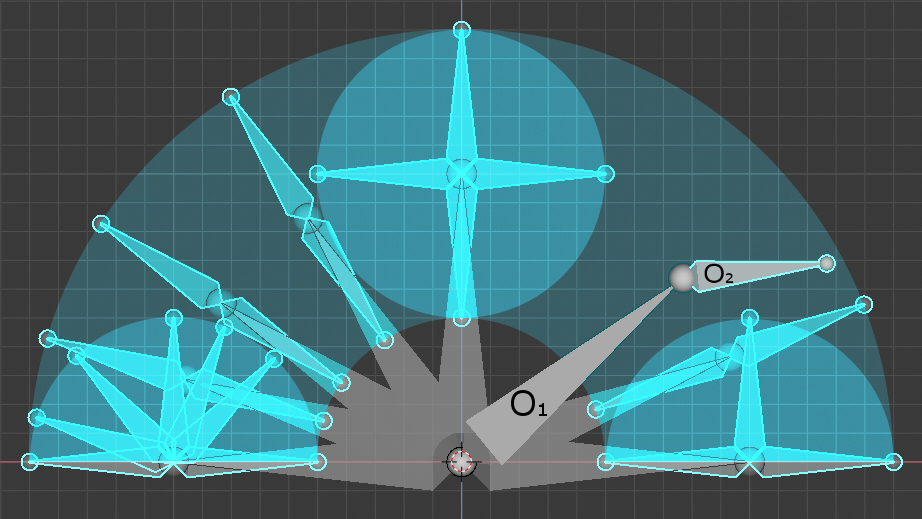
\includegraphics[width=.8\textwidth]{Figures/2Dlinkage}
\decoRule
\caption[Inverse Kinematic 2D]{Esempio di segmento di scheletro formato da due ossa in uno spazio 2D. Quello evidenziato in azzurro è lo spazio raggiungibile dall'\emph{end-effector}}
\label{fig:IK}
\end{figure}

Il concetto di Inverse Kinematic (IK) è, fondamentalmente l'inverso di Forward Kinematic. In quest'ultimo ogni osso influenza la rotazione di quelli che lo seguono (i.e. figli).
Al contrario, in IK, muovere un osso alla fine di una sequenza (i.e. \emph{end-effector}), influenza la posizione di quelli che lo precedono.
Ciò è molto utile nel caso in cui si vogliano posizionare gli arti di una figura umana, in quanto rende il tutto più intuitivo.
IK serve anche a fare in modo che una serie di ossa mantenga un estremo (i.e. \emph{end-effector}) connesso a qualcosa.
Definite la posizione della mano e della radice (spalla) la posizione delle ossa intermedie viene calcolata automaticamente.
Esistono diverse tecniche per il calcolo degli angoli delle articolazioni intermedie.

Nel caso di articolazioni relativamente semplici è possibile calcolare l'intero spazio delle soluzioni analiticamente, ed individuare tra di esse quelle che soddisfano l'obiettivo.
Ad esempio, nel caso di un sistema di due ossa ($O_1$ e $O_2$) e due articolazioni in uno spazio 2D come in Figura \ref{fig:IK} lo spazio raggiungibile dall'\emph{end-effector} può essere descritto come 
\begin{equation*}
    \{x: |O_1-O_2| \leq x \leq O_1+O_2\}
\end{equation*}
\newpage
Data la posizione $(X,Y)$ obiettivo dell'\emph{end-effector}, se questa cade all'interno dello spazio raggiungibile, è possibile attraverso le formule trigonometriche, ricavare gli angoli delle 2 articolazioni:

FIGURE 5.15 PLACEHOLDER 

\begin{align}
    \arccos{ (\theta _T) } &=  \frac{X}{\sqrt{X^2+Y^2}}\\
    \theta_T &= \arccos{\left(  \frac{X}{\sqrt{X^2+Y^2}} \right)}\\
    \cos{( \theta_1-\theta_T )} &=  \frac{O_1^2+X^2+Y^2-O_2^2}{2O_1\sqrt{X^2+Y^2}}\\
    \theta_1 &= \arccos{\left(  \frac{O_1^2+X^2+Y^2-O_2^2}{2O_1\sqrt{X^2+Y^2}}\right)}+\theta_T\\
    \cos{(180-\theta_2)} = -\cos{(\theta_2)} &= \frac{O_1^2+O_2^2-(X^2+Y^2)}{2O_1O_2}\\
    \theta_2 &= \arccos{\left(\frac{O_1^2+O_2^2-X^2+Y^2}{2O_1O_2}\right)}
\end{align}

Nell'equazioni sopra riportate $\theta_1$ e $\theta_2$ si riferiscono agli angoli rispetto alla posizione naturale dei rispettivi ossi.
$\theta_T$ è l'angolo formato dall'ipotenusa immaginaria che si forma tracciando un segmento dalla radice alla posizione obiettivo dell'end-effector, rispetto alla posizione naturale di $O_1$.

Per casi più complessi, come spesso capita nelle animazioni digitali, viene usato un metodo iterativo  analogo alla risoluzione di un problema di ottimizzazione in programmazione lineare \cite{lp2017}, in cui la funzione obiettivo è data dalle variabili che compongono la posizione e l'orientamento dell'end-effector.

\subsection{Lo Jacobiano}

Molti meccanismi di utilizzati nell'ambito delle animazioni digitali sono troppo complessi per essere risolti analiticamente.
Per questi, il movimento può essere costruito in maniera incrementale.
Ad ogni intervallo temporale dell'iterazione, viene calcolato in che modo cambiare gli angoli di ogni articolazione per far sì che la posizione e l'orientamento corrente dell'end-effector si avvicini a quella desiderata.
Per fare ciò esistono diversi metodi \cite{simplex2011, simplex2006} \cite{mingozR2019} \cite{mingozD2019}, molti dei quali utilizzano una matrice di derivate parziali chiamata lo Jacobiano, o matrice Jacobiana.

Per spiegare lo Jacobiano da un punto di vista matematico, si considerino le sei funzioni rappresentate in Equazione \ref{eq:linear}, ciascuna delle quali è una funzione in sei variabili indipendenti tra loro.
Dati i valori di input per le variabili $x_i$, ciascun valore di output $y_i$ può essere calcolato dalla rispettiva funzione $f_i$.
\begin{equation} \label{eq:linear}
    \begin{aligned}
        y_1 = f_1(x_1,x_2,x_3,x_4,x_5,x_6)\\
        y_2 = f_2(x_1,x_2,x_3,x_4,x_5,x_6)\\
        y_3 = f_3(x_1,x_2,x_3,x_4,x_5,x_6)\\
        y_4 = f_4(x_1,x_2,x_3,x_4,x_5,x_6)\\
        y_5 = f_5(x_1,x_2,x_3,x_4,x_5,x_6)\\
        y_6 = f_6(x_1,x_2,x_3,x_4,x_5,x_6)
    \end{aligned}
\end{equation}

Queste equazioni possono anche essere usate per descrivere il cambiamento nelle variabili di output relativo alle variabili di input.
I differenziali di $y_i$ possono essere scritti in termini dei differenziali delle $x_i$ utilizzando la regola della catena, generando l'Equazione \ref{eq:diff}.
\begin{equation}\label{eq:diff}
    dy_i = \dfrac{\partial f_i}{\partial x_1}dx_1+
        \dfrac{\partial f_i}{\partial x_2}dx_2+
        \dfrac{\partial f_i}{\partial x_3}dx_3+
        \dfrac{\partial f_i}{\partial x_4}dx_4+
        \dfrac{\partial f_i}{\partial x_5}dx_5+
        \dfrac{\partial f_i}{\partial x_6}dx_6
\end{equation}
Le Equazioni \ref{eq:linear} e \ref{eq:diff} possono essere possono essere rappresentate in forma vettoriale, producendo le equazioni \ref{eq:vecLin} e \ref{eq:vecDif}, rispettivamente.
\begin{align}
    \label{eq:vecLin}
    dY =  \dfrac{\partial F}{\partial X}dX\\[5ex]
    \label{eq:vecDif}
    dY =  \dfrac{\partial F}{\partial X}dX
\end{align}

Una matrice di derivate parziali, $\frac{\partial F}{\partial X}dX$, viene chiamata \emph{Jacobiana} ed è una funzione dei valori correnti delle $x_i$. Lo Jacobiano può essere visto come l'associamento delle velocità (ad intervallo di tempo regolare) $X$ alle velocità $Y$ (Eq. \ref{eq:velocity}).
\begin{equation}\label{eq:velocity}
    \dot{Y} = J(X)\dot{X}
\end{equation}

In qualunque momento, lo Jacobiano è una funzione delle $x_i$. All'iterazione successiva, $X$ sarà cambiata e, allo stesso modo lo sarà la trasformazione rappresentata dallo Jacobiano.

Quando si applica lo Jacobiano ad una catena di ossa, le variabili di input, $x_i$, rappresentano i valori delle articolazioni, e le variabili di output, $y_i$, quelli dell'end-effector (reppresentati come angoli $x,y,z$).
\begin{equation}
    Y=
    \begin{bmatrix}
        p_x & p_y & p_z & \alpha_x & \alpha_y & \alpha_z
    \end{bmatrix}
    ^T    
\end{equation}

In questo caso, lo Jacobiano associa le velocità degli angoli delle articolazioni, $\dot{\theta}$, alle velocità della posizione e orientamento dell'end-effector, $\dot{Y}$ (Eq. \ref{eq:Jangle}).
\begin{equation}\label{eq:Jangle}
    V = \dot{Y} = J(\theta)\dot{\theta}
\end{equation}

$V$ è il vettore delle velocità lineari e angolari, e rappresenta la trasformazione che si vuole applicare all'end-effector.
Tale trasformazione si basa sulla differenza tra la posizione/rotazione corrente e quella specificata come obiettivo.
Queste velocità sono vettori in uno spazio tridimensionale, pertanto ciascuna ha tre componenti, $x$, $y$ e $z$ (Eq. \ref{eq:Vgoal}).
\begin{equation}\label{eq:Vgoal}
    V=
    \begin{bmatrix}
        v_x & v_y & v_z & \omega_x & \omega_y & \omega_z
    \end{bmatrix}
    ^T
\end{equation}

$\dot{\theta}$ è un vettore delle velocità delle articolazione, in altre parole, contiene i cambiamenti dei parametri di ogni articolazione, ovvero le incognite dell'equazione (Eq. \ref{eq:Vartic}).
\begin{equation}\label{eq:Vartic}
    \dot{\theta}=
    \begin{bmatrix}
        \dot{\theta}_1 & \dot{\theta}_2 & \dot{\theta}_3 \ldots \dot{\theta}_n
    \end{bmatrix}
    ^T
\end{equation}

La matrice Jacobiana, $J$, è una matrice che associa i due vettori appena visti, ed è una funzione della posa corrente (Eq. \ref{eq:Jacobian}).

\begin{equation}\label{eq:Jacobian}
    J=
    \begin{bmatrix}
        \dfrac{\partial p_x}{\partial \theta_1} & \dfrac{\partial p_x}{\partial \theta_2} & \dots & \dfrac{\partial p_x}{\partial \theta_n} \\[2ex]
        \dfrac{\partial p_y}{\partial \theta_1} & \dfrac{\partial p_y}{\partial \theta_2} & \dots & \dfrac{\partial p_y}{\partial \theta_n} \\[2ex]
        \vdots & \vdots & \ddots & \vdots \\[2ex]
        \dfrac{\partial \alpha_z}{\partial \theta_1} & \dfrac{\partial \alpha_z}{\partial \theta_2} & \dots & \dfrac{\partial \alpha_z}{\partial \theta_n} 
    \end{bmatrix}
\end{equation}

Ogni termine dello Jacobiano rapporta il cambiamento di una specifica articolazione ad uno specifico cambiamento dell'end-effector.
Per una giuntura rivolutiva (i.e. che ruota su un singolo asse), il cambiamento di rotazione nell'end effector, $\omega$, è semplicemente la velocità angolare dell'articolazione intorno all'asse di rotazione per la giunzione che si sta considerando.
Per un'articolazione prismatica, in cui un osso trasla rispetto al padre, la rotazione dell'end-effector rimane inalterata dal cambiamento nell'articolazione.
Per un'articolazione rotazionale, la trasformazione lineare nell'end-effector è il risultato del prodotto vettoriale tra l'asse di rivoluzione e il vettore che parte dall'articolazione, fino all'end-effector.
La rotazione di un articolazione rotazionale induce uno spostamento istantaneo dell'end-effector.
Per un'articolazione prismatica, lo spostamento equivale a quello dell'articolazione (vedi Fig. \ref{fig:velocities}).

FIGURE 5.16 PLACEHOLDER\label{fig:velocities}

Le velocità lineari e angolari desiderate sono calcolate trovando la differenza tra la configurazione dell'end-effector corrente e quella obiettivo. Le velocità indotte dalla rotazione di una specifica articolazione, sono determinate dai calcoli mostrati in Figura \ref{fig:velocities}.
Il problema sta nel determinare la migliore combinazione lineare delle velocità, indotte dalle varie articolazioni, che risulti nelle velocità desiderate nell'end-effector.
Lo Jacobiano è il risultato della rappresentazione del problema descritto, in forma di matrice.

È importante che, nel rappresentare il problema in forma Jacobiana, tutte le coordinate dei valori delle articolazioni, siano rappresentate come coordinate dello stesso sistema (e.g. coordinate globali).
Spesso infatti, le informazioni relative ad una particolare articolazione sono rappresentate nel sistema di coordinate locale a quell'articolazione.
Durante la creazione della matrice Jacobiana, queste informazione devono essere convertite in un sistema di coordinate comune, come quello delle coordinate globali, o dell'end-effector.
Esistono diversi metodi per calcolare lo Jacobiano che si basano sul massimizzare l'efficienza computazionale date le informazioni in coordinate locali, tutti però producono il risultato in un sistema di coordinate comune.

FIGURE 5.17 PLACEHOLDER\label{fig:IKex0}

Per fare un esempio inerente a questo progetto, si consideri lo scheletro di uno qualunque dei personaggi, in particolare il suo braccio.
In questo caso ci si può limitare ad un movimento in un piano fissato, che quindi esclude dal problema una delle tre dimensioni e vincola le rotazione ad un unico asse ($z$).
In Figura \ref{fig:IKex0} si vuole spostare l'end-effector, rappresentato dal polso ($A_2$), nel punto $P$. In questo caso particolare, l'orientamento della mano non ha importanza.
L'asse di rotazione di ogni articolazione ($A_i$) è perpendicolare alla figura ed esce dal foglio.
L'effetto di una rotazione incrementale, $r_i$, di ciascuna articolazione, è dato dal prodotto vettoriale tra l'asse dell'articolazione e il vettore che collega quest'ultima all'end-effector, $\vec{V_i}$ (vedi Fig \ref{fig:IKex1}), e costituisce le colonne della matrice Jacobiana.
È importante notare come ogni rotazione di un'articolazione influenzi tutte quelle successive. Di conseguenza, le prime hanno un'intensità maggiore rispetto alle ultime ($r_1>r_2>r_3$). In termini tecnici la lunghezza di ogni $r_i$ è funzione della distanza tra la posizione della rispettiva articolazione dall'end-effector.

FIGURE 5.18 PLACEHOLDER\label{fig:IKex1}

La trasformazione da applicare all'end-effector è il risultato della differenza tra la sua posizione corrente e quella obiettivo (Eq. \ref{eq:Vresult}).
\begin{equation}\label{eq:Vresult}
    V=
    \begin{bmatrix}
        (P - A_2)_x\\
        (P - A_2)_y\\
        (P - A_2)_z
    \end{bmatrix}
\end{equation}

Il vettore delle trasformazioni che si vogliono applicare è uguale alla matrice Jacobiana (Eq. \ref{eq:Jresult}) moltiplicata per il vettore delle incognite, date dali cambiamenti negli angoli delle articolazioni.
\begin{equation}\label{eq:Jresult}
    J=
    \begin{bmatrix}
        \big((0,0,1) \times A_2\big)_x & \big((0,0,1) \times A_1\big)_x\\
        \big((0,0,1) \times A_2\big)_y & \big((0,0,1) \times A_1\big)_y\\
        \big((0,0,1) \times A_2\big)_z & \big((0,0,1) \times A_1\big)_z
    \end{bmatrix}
\end{equation}

Una volta calcolato lo Jacobiano, bisogna risolvere un'equazione nella forma mostrata in Equazione \ref{eq:J+1}. Nel caso $J$ sia una matrice quadrata, l'inversa dello Jacobiano, $J^{-1}$, può essere utilizzata per calcolare le velocità angolari delle articolazioni, date quelle dell'end-effector (Eq. \ref{eq:J-1}).
\begin{align}
    \label{eq:J+1}
    V &= J\dot{\theta}\\
    \label{eq:J-1}
    J^{-1}V &= \dot{\theta}
\end{align}

Blender propone due metodi per risolvere la cinematica inversa, uno di questi tiene conto anche di altri vincoli definiti dall'utente \cite{blendDoc}. Questo metodo si chiama iTaSC e, come il metodo standard, utilizza una matrice Jacobiana, ma il modo in cui la calcola è differente \cite{blendWiki}.

Un motivo per cui il metodo iterativo è migliore di quello analitico, oltre ad essere l'unico metodo per risolvere articolazioni complesse, è che, nel caso in cui la posizione obiettivo si trovi al di fuori dello spazio raggiungibile, (e.g. la mano deve raggiungere un punto troppo distante dalla spalla) non esiste nessuna soluzione e in questo caso il risultato può e dev'essere approssimato.

Siccome quello della cinematica inversa è un problema sotto-vincolato, è molto probabile che esista più di una soluzione. Nel caso visto in Figura \ref{fig:IK} ad esempio esistono 2 soluzioni, per un qualsiasi punto $(X,Y)$ interno allo spazio raggiungibile, simmetriche rispetto alla linea immaginaria che collega la radice di $O_1$ alla punta di $O_2$.
In tal caso il risultato è scelto dall'algoritmo tra una delle possibili soluzioni. Non sempre però, sono tutte realistiche o visivamente gradevoli.
Per questo motivo è possibile aggiungere dei vincoli per limitare il numero di soluzioni possibili, molto utili sono quelli per l'imitare il movimento di un arto, per renderlo più realistico.


